%!TEX root = ../thesis.tex
%*******************************************************************************
%*********************************** First Chapter *****************************
%*******************************************************************************

\chapter{Introduction}

\ifpdf
    \graphicspath{{Chapter1/Figs/Raster/}{Chapter1/Figs/PDF/}{Chapter1/Figs/}}
\else
    \graphicspath{{Chapter1/Figs/Vector/}{Chapter1/Figs/}}
\fi

\section{Genetic variation}

\par{
Even before Gregor Mendel discovered the rules of genetic inheritance\cite{mendel}, the discovery that DNA was the molecule responsible for this\cite{Avery}, or its structure was known\cite{watsoncrick}, humans have wondered at the variation among each other and all organisms. These discoveries have since made way for a rapid expansion in our ability to measure genetic variation from capillary sequencing\cite{capillary} and single nucleotide polymophism (SNP) chips\cite{snpchip} to modern high throughput DNA sequencing\cite{bridgeamp} and long read sequencing\cite{HIFI}. We have sequenced thousands of individual humans and other organisms and explored the genetic variation of the human species \cite{1kgenomes}\cite{1kgenomes2}\cite{haplotypepanel}\cite{ukbiobank}\cite{hapmap}. We have used the genetic variation in population samples to impute population structure and evolutionary history\cite{NGSadmix}\cite{angsd}\cite{estimateadmixture}\cite{abbababa}\cite{shapeit4}\cite{beagle}. In this thesis, I explore computational methods for using genetic variation to resolve mixtures of haplotypes in single cell RNAseq, genome assembly, and scaffolding.
} \\ 

\section{Introductiion}

\par{
In single cell RNA sequencing, the goal is not only to measure the transcriptome of many cells at a time, but also to compare the transcriptome of cells of different individuals or under different conditions such as disease state, pharmaceutical intervention, or a wide range of environmental differences. One problem with these comparisons is that there can be technical artifacts, or batch effects, between different experiments which bias the comparative results possibly even dwarfing the actual biological difference you are trying to measure. One solution to this problem is to pool the cells from different individuals into a single experiment. Additionally, single cell RNAseq has several sources of noise or errors (discussed in more detail in section \ref{section:scerrors}). One is when two or more cells are erroneously partitioned into the same compartment and the data for what is supposed to be one cell is actually two cells (doublets). And another source of noise is when RNA from previously lysed cells which are in solution with the cell suspension is sequenced along with the RNA from a patent cell and those reads are given the same cellular barcode (ambient RNA). In Chapter 2 of this thesis, I present a method for demultiplexing cells from mixtures of individuals into their individual of origin using the genetic variation measured in the single cell RNAseq reads without requiring prior knowledge of the genotypes. In addition, I show how---and provide methods for---how these mixtures improve doublet detection and ambient RNA estimation and removal.
} \\

\begin{figure}[htbp!]
\begin{centering}

\caption{Outline of single cell clustering by genotype}\label{fig:souporcell}
\sidesubfloat[]{
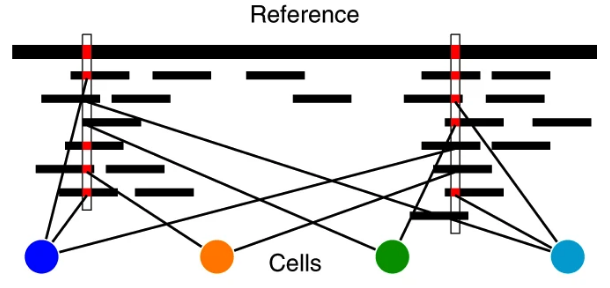
\includegraphics[width=0.3\textwidth, valign=c]{cellvariant.png} \label{fig:a}
}
\sidesubfloat[]{
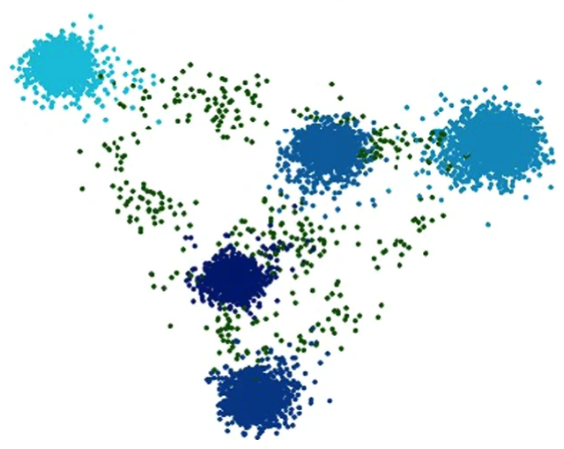
\includegraphics[width=0.3\textwidth, valign=c]{cellclust.png} \label{fig:b}
}
\sidesubfloat[]{
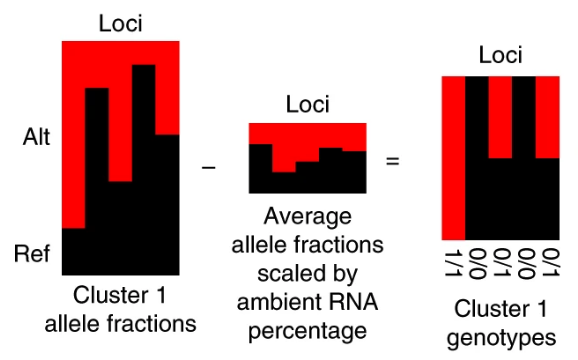
\includegraphics[width=0.3\textwidth, valign=c]{ambientrna.png} \label{fig:c}
}
\par{\textbf{a)} We find the variants in the reads from each cell barcode, \textbf{b)} cluster cells by their allele content and identify doublets, and \textbf{c)} use the bias in allele fraction from expected values to estimate and remove ambient RNA.}
\end{centering}
\end{figure}

\par{
In genome assembly, the goal is the use the overlapping read sequence similarity to infer that those reads came from the same locus in the genome and build contiguous sequences that represent (in part or whole) the organism's chromosomes. The inference that sequence similarity means these reads originated from the same genomic locus is complicated by repeats, heterozygosity, and sequencing errors. With inexact homology, one must disambiguate whether the differences arose from errors, paralogous repeat sequences, or from the alternate haplotype. If one cannot make this distinction and no reads span this region into more unique sequence, the contiguous sequence (contig) must be broken resulting in a fractious assembly. If the contig is not broken, one risks a chimeric misassembly of sequences that are distant to one another in the genome or on different chromosomes being assembled close to one another. In chapter 3 we discuss the first high quality assembly of a single mosquito. Prior to this, long read sequencing methods (discussed in section \ref{section:longreads}) DNA input requirement were too high to extract enough high molecular weight (HMW) DNA from many small organisms including mosquitos. This required pooling multiple individuals together in order to meet the DNA requirements for these sequencing technologies. Pooling individuals increases the number of haplotypes in the extracted DNA and makes distinguishing repeat from heterozygosity harder. Through recent advances in library preparation, the DNA requirements for long reads has been greatly reduced. By sequencing a single mosquito with long reads, we reduce the number of haplotypes from many down to two thus decreasing the potential ambiguities that arise from heterozygosity. We then compare this genome assembly to the current gold standard assembly of \textit{Anopheles gambiae} which was created using Sanger sequencing and bacterial artifical clones (discussed in section \ref{section:sanger} and \ref{section:BACs}), a dramatically higher cost method of creating high quality genome assemblies. We show many improvement in our assembly over the previous gold standard as well as highlight several issues that remain with the current assembly state of the art.
} \\



\par{
We continue to address the problem of heterozygosity in chapter 4 by showing several ways in which haplotype phasing consistency can be used as a signal for physical linkage. Given two or more proximate heterozygous loci, sequencing reads containing them should segregate into two groups according to which alleles they contain (assuming diploid). But how do we know that a site is heterozygous. Initially we do not. We can find sequence which has inexact homology each being read roughly half of the times general homozygous sequences occur. These could be due to heterozygosity or paralogous sequences both with low occurrence by chance due to random sampling. In both cases, reads containing multiple of these alleles should segregate into two (assuming copy number of the repeat is two) groups. But when comparing a true heterozygous site with inexact homologous sequence caused by paralogous sequence, the reads with both alleles of the heterozygous site will contain one of the presumed alleles caused by the repeat sequence. We can use this property in both assembly and scaffolding to avoid misassemblies, create phased assemblies, and scaffold contigs in a phasing aware fashion. In chapter 4, we outline how we go about finding candidate heterozygous sequences in a \textit{de novo} way, the phasing consistency criteria, how we build a phased assembly graph, and can separate reads by their haplotypes prior to haploid assembly. We also show how to use this same property for scaffolding using long range genetic information from linked reads and HiC (discussing in sections \ref{section:linkedreads} and \ref{section:hic}). In case the assembly we wish to scaffold was not built by our phased assembly method, we also provide an algorithm for haplotype phasing the \textit{de novo} candidate heterozygous sites within each contig which is a requirement for phasing aware scaffolding. This tool has the added benefit of being robust to being given non heterozygous sequences as input and can use the phasing inconsistency to correct the genotypes. We demonstrate these techniques on data from the butterfly \textit{Vanessa atalanta}.
} \\

\begin{figure}[htbp!]
\begin{centering}

\caption{Phasing consistency as a \textit{de novo} signal for physical linkage}\label{fig:phasstools}
\sidesubfloat[]{
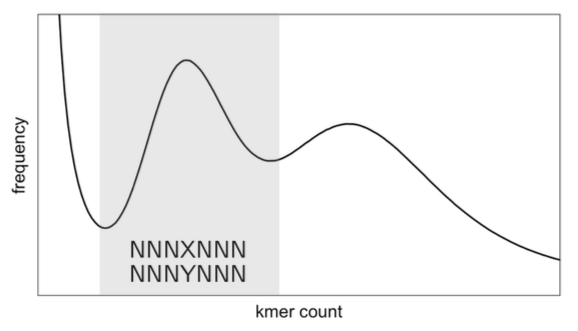
\includegraphics[width=0.3\textwidth, valign=c]{spectrum.png} \label{fig:a}
}
\sidesubfloat[]{
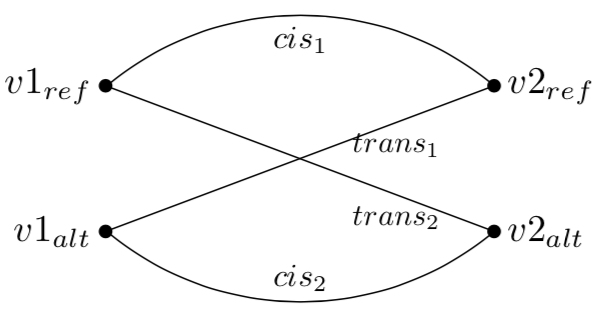
\includegraphics[width=0.3\textwidth, valign=c]{consistency2.png} \label{fig:b}
}
\sidesubfloat[]{
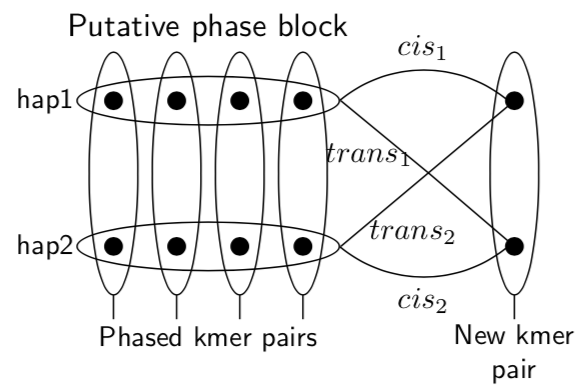
\includegraphics[width=0.3\textwidth, valign=c]{consistency3.png} \label{fig:c}
}
\par{\textbf{a)} We use the kmer count spectra to determine candidate heterozygous kmer pairs which we can then \textbf{b)} assess for phasing consistency based on the alleles on reads that contain one of each, and \textbf{c)} build a phased assembly graph.}
\end{centering}
\end{figure}

\par{
The remainder of this chapter contains the background and context for this work. I first cover the history of single cell sequencing and analysis. I then outline the biases and errors that occur in single cell sequencing and the various solutions and their downsides which motivates chapter 2. I then go over the history of DNA sequencing methods as well as assembly and scaffolding algorithms. I discuss the inherent ambiguities that can occur and the errors that can arise and their causes which motivates chapters 3 and 4.
}

\section{Single Cell RNAseq}

\par{
The etymology of the word cell comes from the latin \textit{cella} meaning storeroom or chamber. These entities separate the physical space between what is life and nonlife, first discovered by Robert Hooke in 1665\cite{Hooke}. This partitioning the cell provides is necessary for life due to the second law of thermodynamics and the nature of life. In Erwin Schrodinger's classic lecture series and book titled ``What is Life"\cite{whatislife}, he noted that while closed physical systems will always tend toward increased entropy (stated by the 2nd law of thermodynamics\cite{thermodynamics1}\cite{thermodynamics2}\cite{maxwell}), life must maintain (on average) a neutral or negative entropy in the portion of the system in which it resides\cite{informationtheorylife}\cite{astrobiology}\cite{extremalities}. In order to do so, this requires the expenditure of energy. Biological evolution found an economical way of solving this problem with the bilipid membrane with various embedded molecules giving it the property of semipermeability---allowing some molecules in and not out or vice versa in a dynamic fashion. These cells proved, over time, to be so successful as to become the primary unit and building block of biological life on this planet. Incidentally, Erwin Schrodinger, as the father of quantum mechanics, along with Josiah Gibbs, as the father of statistical mechanics, will appear several times in this thesis as some of the algorithms described take ideas inspired by these fields for search strategies in optimization methods.
} \\

\par{
When studying the state of a cell and its current function, we could try to measure many different properties such as the proteome, transcriptome, genome, chromatin accessability, environmental conditions (such as hormone content, PH, etc), cell surface proteins. But we are somewhat limited by the tools available, and when addressing function, we first turn to the central dogma of molecular biology\cite{centraldogma} that states that information in general passes from DNA to RNA and then to proteins. If we could easily inspect the protein content of many cells in a high throughput fashion, that would be desirable, but protein detection and sequencing methods often only limited to one or a few proteins at a time and/or are not high throughput\cite{immunohistochemistry}\cite{multiIHC}\cite{westernblot}\cite{western2}\cite{multimassspec}\cite{ionbeam}\cite{cellIHC}\cite{proteinsequencing}. But we do have a very high throughput detector for DNA and can convert RNA into complementary DNA (cDNA).
}

\subsection{Bulk RNAseq}
\par{
Scientists have been sequencing cDNA libraries of RNA isolated from many cells mixed together since the advent of next generation DNA sequencing technologies (discussed in section \ref{section:nextgen}) became available\cite{RNAseq1}\cite{RNAseq2}. Because these use extractions from pools of cells, they are denoted as `bulk' RNAseq. These experiments have provided many discoveries, but are limited in their usefulness because they represent the average transcriptome across a population of potentially diverse cells. This blurs the data and makes inference on minority cell types difficult if not impossible. The amount of RNA in a single cell is roughly 10-30pg\cite{howmuchrna} which until recently was not enough to create a complex cDNA library from even with amplification. Some researchers have isolated specific cell types using Fluorescence Activated Cell Sorting (FACS)\cite{FACspatent}\cite{FACs} prior to RNAseq to some success\cite{FACszebra}, but due to FACS cell stress and it only accessing one cell type at a time it is of limited usefulness.
}

\subsection{Single cell RNA sequencing}

\par{
In the past decade, technical advances in methods for the preparation of samples containing minuscule amounts of nucleic acids have made it possible to study the transcriptome of single cells\cite{first_singlecell} and have changed the way biologists can access the functional state of individual cells within a complex and diverse population of cells in tissues across different states of organisms shedding light on the cellular response to diseases, drugs, development, and more.
} \\
\par{
There are many types of RNA in the cell including messenger RNA (mRNA), transfer RNA (tRNA), ribosomal RNA (rRNA), micro RNA, and small nucleolar RNA. mRNA makes up only 3-7\% of the cell's total RNA by mass\cite{rnacontent}, but it is what is translated by ribosomes into proteins, which conduct a large amount of the function of the cell. Single cell RNA sequencing targeting other types of RNA have also been developed for alternative types of RNA for specific purposes\cite{nonmRNASC}, but in this thesis when referring to single cell RNAseq (scRNAseq) we are talking about a system that enriches for mRNA by using the 3' polyadenylation most mRNAs have (with some exceptions\cite{nonpoly}).
}

\subsection{Technologies}

\par{
mRNA from a single cell was first isolated and amplified to measurable levels with polymerase change reaction (PCR)\cite{PCR}\cite{PCRPatent} in the early 1990s\cite{earliersinglecell} before the sequencing revolution. Without a high throughput detector, and due to the exponential nature of PCR causing abundant mRNA to dominate the sample, very few genes are detected. This increased with linear amplification achieved by multiple cycles of transcription of antisense RNA from the initial cDNA using T7 RNA polymerase\cite{T7amp} and the advent of oligonucleotide microarrays\cite{snpchip} allowing for RNA microarray studies detecting over a thousand genes\cite{microarrayRNA}\cite{microarraySC2}. However, the number of genes measured were still a fraction of the total genes expressed. The first sequencing of single cell cDNA sequencing increased the number of genes detected by 75\%\cite{first_singlecell} and provided a hypothesis free measurement of the transcriptome a single cell. Since then, single cell RNAseq has grown greatly in the number of cells processed per experiment, the number of genes detected per cell, and its uptake by the scientific community\cite{singlecellgrowth}.
}

\par{
Current scRNAseq protocols convert RNA to cDNA using a reverse transcriptase primed off of the poly-A tail of the mRNA. At the same time, a cellular barcode as well as template switching oligo (for subsequent PCR) are added. Often, a unique molecular identifier (UMI) is also added. This is used to know which cDNA molecules were amplified from the same RNA source molecule to avoid counting PCR duplicates multiple times\cite{UMI1}\cite{UMI2}. This reduces the PCR biases versus a simple read counting strategy. 
} \\

\par{
To deliver a barcode oligo to all of the reads originating from one cell and different barcodes to different cells, physical separation of one form or another is generally used. The separation could be in different tubes, plate wells, nanowells\cite{seqwell}\cite{scalablemicro}\cite{combilabel}, or more recently with microfluidic systems creating a reverse emulsion droplets\cite{dropseq}\cite{Klein2015}\cite{10xsinglecell}. These methods vary in several parameters including the scalability of number of cells per experiment, the capture rate of mRNA, and the technical variation between experiments among others\cite{powersingle}\cite{singlecompare}\cite{singlecompare2}. Which method is best to use ultimately depends on the biological question. For experiments where sampling the whole population of cells is important, droplet and nanowell methods are better whereas if capture rate and amount of data per cell, plate based systems would be better. 
}

\subsubsection{10x genomics}

\par{
In this thesis, all of the single cell data used was generated using the 10x genomics chromium platform, a reverse emulsion droplet based system. Figure \ref{figure:10xsinglecell} outlines how this system works. It uses a microfluidic system to deliver gel beads, reagents, and cells into reverse emulsion droplets where the reverse transcription occurs. The gel bead contains oligos with the cell barcode, a UMI, and primers for the PCR and Illumina sequencing\cite{10xsinglecell}.
}
\begin{figure}[htbp!]
\caption{10x Genomics single cell RNAseq}
\label{figure:10xsinglecell}
\begin{centering}
\sidesubfloat[]{
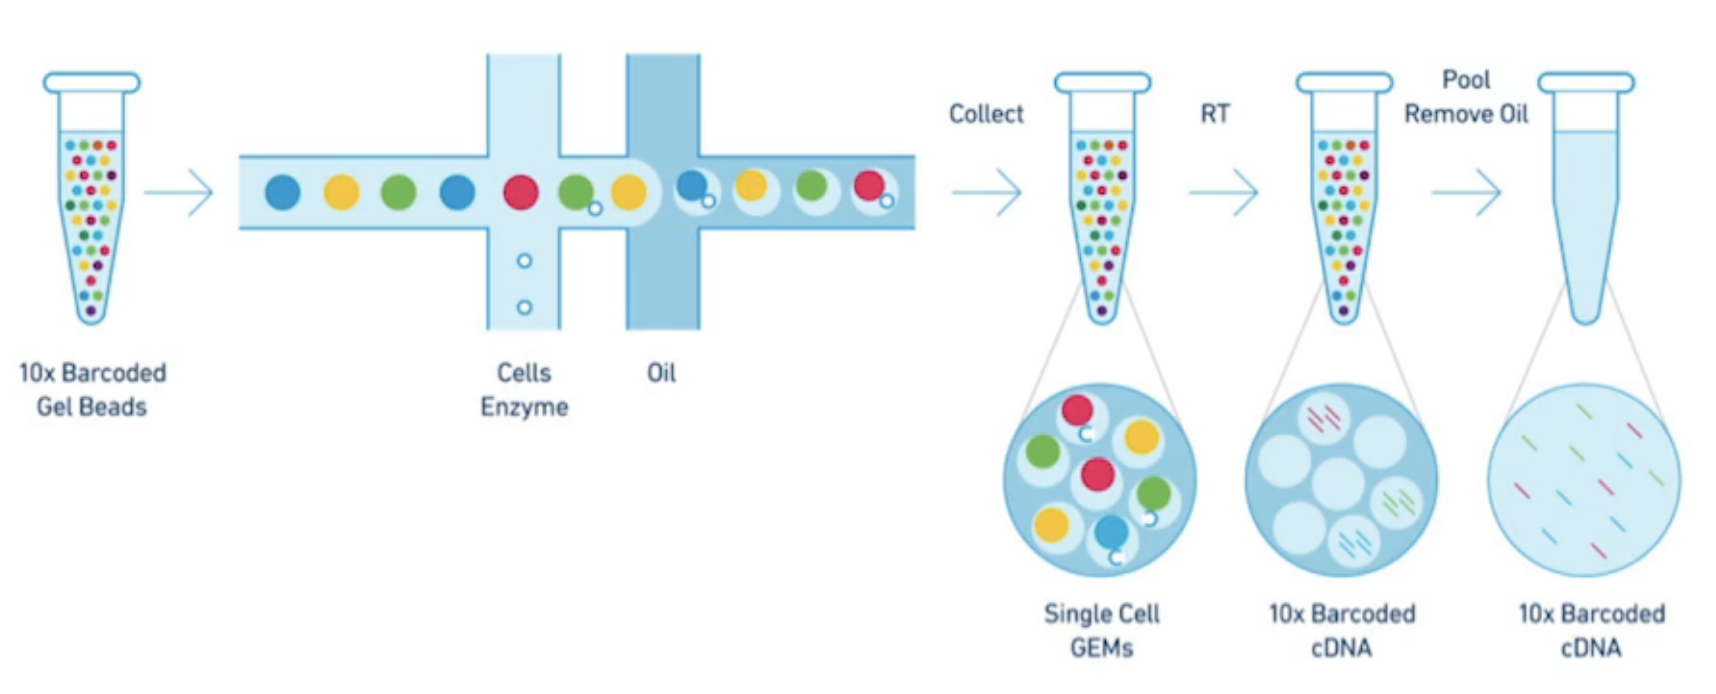
\includegraphics[width=0.85\textwidth]{singlecelloverview2.png}} \\
\sidesubfloat[]{
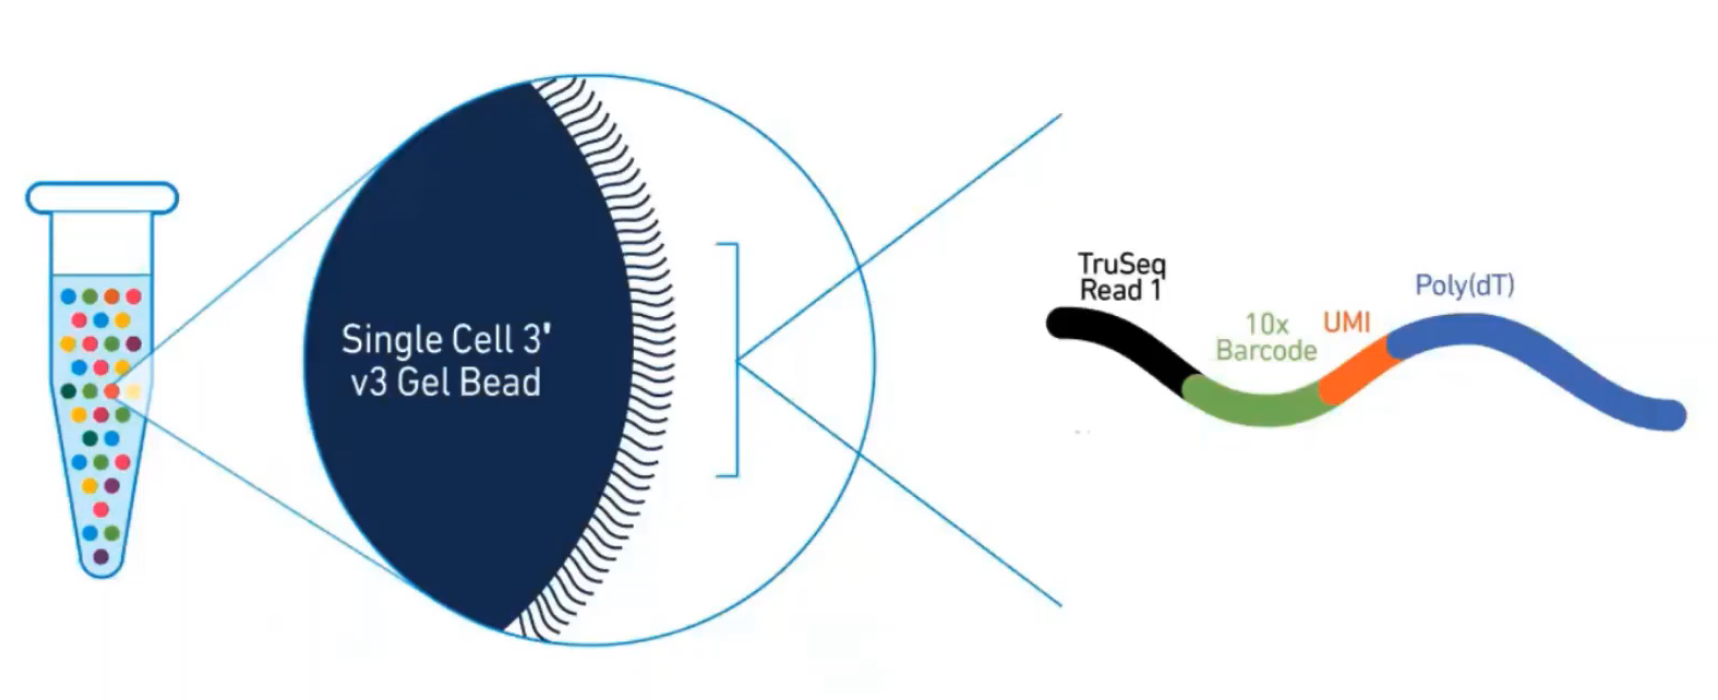
\includegraphics[width=0.85\textwidth]{singlecell2.png}
}
\par{Diagram outlining 10x Genomics single cell sequencing technology (credit: 10x genomics website).}
\end{centering}
\end{figure}

\subsection{Analysis of scRNAseq data}

\par{
This construct is then sequenced on a next-generation Illumina sequencer \cite{bridgeamp}\cite{illuminareview} (discussed in detail in section \ref{section:nextgen}) giving paired-end reads with one read containing the cell barcode and UMI and the other read containing the cDNA of the mRNA transcript. Other sequencing platforms have been used, notably long read sequencing platforms to get the whole transcript read to investigate alternative isoforms, but will not be discussed further here\cite{tilgner}\cite{isoformseq}\cite{longreadsinglecell}. The most common software package used to go from the sequence files to cell gene counts matrix and initial cell type clustering is cellranger\cite{cellranger} and while alternatives exist\cite{dropseqsoft}, they do largely the same steps. 
}

\subsubsection{Genome alignment}

\par{
First, the template switch oligo and polyadenylation are trimmed from the 5' and 3' ends of read two respectively. Then the read two is mapped to the given reference genome using the STAR splicing aware RNA aligner\cite{STAR}. Other aligners exist for this purpose such as HISAT2 \cite{hisat} and TopHat2 \cite{tophat2}. Also there are psuedo-aligners (Kallisto\cite{kallisto} and Salmon\cite{salmon}) which are much faster and robust to sequencing errors but do not provide spicing information\cite{alignfree}. The reads are then marked as exonic or intronic using the given transcript annotation gene transfer format (GTF) file and confident or not based on if the read overlaps an exon for >50\% of its length and if the mapping quality (mapq) is 255 which indicates that the read aligned uniquely to one location. Confident exonic reads are carried forward to the UMI counting step\cite{singlecelloverview}.
}

\subsubsection{Barcode correction}
\par{
Before counting UMIs, cellranger attempts to do barcode correction on the cell barcodes. 10x Genomics uses a designed barcode set of either 737 thousand or 3 million barcodes each with a hamming distance\cite{hamming} of at least two to any other barcode in the set. The barcodes that make up this designed set are the barcodes we expect to see and this set is termed the whitelist. In order to error correct barcodes, first the frequency of each barcode in the whitelist is counted. Then for every barcode that is not in the whitelist, each sequence that is one hamming distance from this sequence and is on the barcode is found. A posterior probability is computed with the priors set by the frequency of that whitelist barcode and the base quality of the changed base used to determine likelihood of that error. For a barcode correction to then take place, the posterior probability of that whitelist barcode must be over 97.5\%\cite{barcodecorrection}.
}

\subsubsection{UMI counting}

\par{
PCR duplicates are then removed using the cell barcode, UMI, and gene. If any reads have the same three, all are discarded except one. The remaining reads will be counted to create the cell barcode by gene count matrix. Note that not each cell barcode contains a cell. Due to ambient RNA in solution from cells lysed before reverse emulsion partitioning, droplets without a patent cell will have some reads. We next need to determine which cell barcodes have cells and which do not.
}



\subsubsection{Cell-barcode detection}
\par{
Initially, cell containing GEMs were called using the second derivative of the log-log UMI counts by barcodes plot (see figure \ref{figure:knee}). More recently, a method using the RNA content of the confidently empty droplets called EmptyDrops\cite{emptydrops} was developed to compare that RNA content (which is generally an average of the RNA content of all cells assuming each cell type lyses with equal probability) with the RNA content of the cells to determine an appropriate cutoff where the difference from the average decreases rapidly. This particularly helps in situations where the cell population contains some cells with a large amount of transcription and another cell type with many fewer transcripts. Both of these cell types will likely still have a very different transcriptional profile than the empty droplets. This algorithm has now been implemented in cellranger. The raw cell barcode by genes UMI counts matrix is then filtered to retain only cell containing cell barcodes.
}
\begin{figure}[htbp!]
\caption{Cell barcode detection knee plot old vs new algorithm}
\label{figure:knee}
\begin{centering}
\sidesubfloat[]{
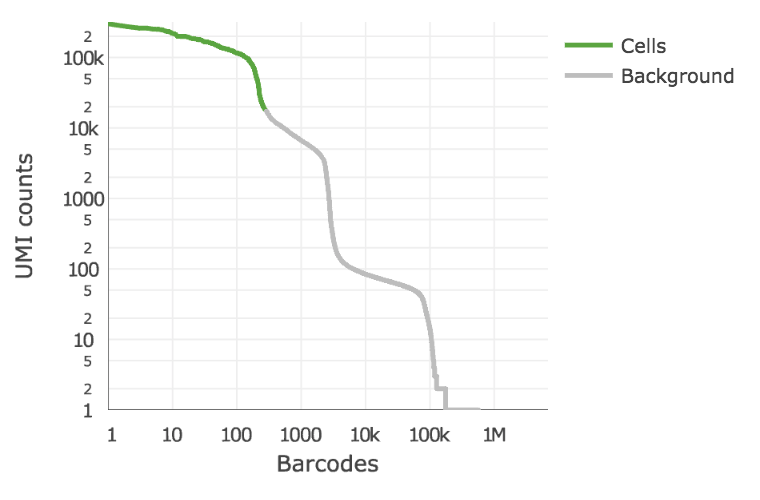
\includegraphics[width=0.45\textwidth]{knee1.png}} 
\sidesubfloat[]{
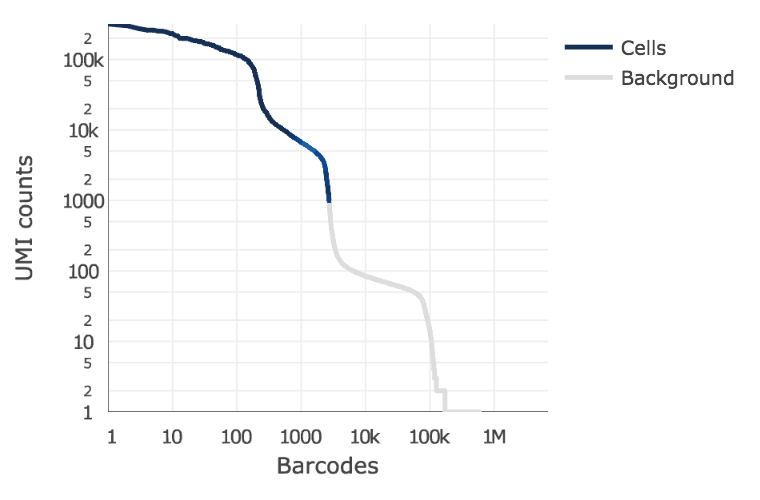
\includegraphics[width=0.45\textwidth]{knee2.png}
}
\par{Log-log barcode by UMI count knee plots showing which barcodes were determined to contain cells under the \textbf{a)} old method using 2nd derivative and the \textbf{b)} new EmptyDrops method (credit: 10x genomics website).}
\end{centering}
\end{figure}

\subsubsection{Quality control}

\par{
Many of the following steps are done in software packages downstream from cellranger which aim to implement many types of analyses for scRNAseq data. The most popular of these software packages is seurat\cite{seurat1}\cite{seurat2} and while alternatives such as Monocle\cite{monocle}, a comparison is out of the scope of this thesis.
} \\

\par{ In the process of cell dissociation, liquid handling, and partitioning, some cells may be damaged. For this reason, many researchers use different criteria to remove these poor quality cells. Some also use different criteria for different cell types and so a less stringent global filter may be applied prior to cell type detection and further filtering. These criteria include number of genes per cell, \% mapped reads, \% reads that map to spike in controls, \% mitochondrial reads, and \% of reads that are PCR duplicates. While these are reasonable markers for dead or dying cells\cite{osorio}\cite{ilicic}, it is my personal opinion that this type of quality control should be limited and standardized as much as possible to prevent unintentional bias in the results affecting how these thresholds are chosen. 
}

\subsubsection{Normalization}

\par{
As previously discussed, individual cells have extremely small amounts of mRNA and require methods to amplify this material in order to be made into a cDNA library and sequenced. These methods, along with the innate difficulties of measuring such a small amount of starting material inevitably result in some technical artifacts. Genes that are expressed to a lesser degree than other genes may show zero counts or lower than true counts in the experiment for several reasons\cite{technoise}. Capture rate of mRNA in the reverse transcription step will never have complete yield and may vary from cell to cell and gene to gene. Additionally, genes that are expressed might be made into cDNA and amplified, but not sampled in the sequencing step as transcripts that begin with a higher copy number get amplified more in the exponential PCR step. Differences in cell size, and thus mRNA content, may result in sampling of genes in one cell type not sampled in other cell types even if both express them. To address this, many normalization methods have been developed\cite{normalize1}\cite{normalize2} to address these problems. Spike in controls can be used to improve this normalization\cite{marioni1} but takes up valuable sequencing. Another solution is imputation\cite{imputesc}, but this can introduce unwanted false positives\cite{fpimpute}. In the comparison papers, differential expression has been shown to be the downstream application most sensitive to these methods\cite{normalsc}, with scran\cite{scran} performing the best of those tested.
}

\subsubsection{Visualization}

\par{
In order to visualize this high dimensional data, we must project it into two or three dimensions in a way that preserves the biologically interesting structure at multiple scales. First, a principle component analysis (PCA) of the filtered cell by genes counts is done to find the most meaningful features and reduce the dimensionality from cells x genes to cells by $M$ where $M$ is a user settable value\cite{pcaimpl}. For most experiments, the complexity of the transcriptional profile cannot be easily gleaned by looking at the first two-three principle components visually, so the next step is to use non-linear dimensionality reduction techniques to bring the data into a visually informative two or three dimensional space. The two most popular methods for this are the t-Stochastic Neighbor embedding (t-SNE)\cite{tsne1}\cite{tsne2}\cite{hinton} and the Uniform Manifold Approximation and Projection (UMAP)\cite{umap1}. Both of these methods aim to preserve pairwise distances in the final projections, but are parametric and non-deterministic (without a fixed psuedorandom number generator seed). There is an inherent trade-off between how well distances should be preserved at different scales which the parameters can help guide. However, due to the randomness and parametric nature of these algorithms, it can lead some researchers to use them to bias the results toward the expected outcome of their hypothesis. Nonetheless, these are powerful techniques to understand high dimensional data such as single cell RNAseq. Recently, UMAP has grown in popularity over t-SNE because it has been shown to better preserve pairwise distance due to the improved initialization strategy employed in the primary implementation and is more computationally efficient than t-SNE\cite{umap2}\cite{umap3}. These projections are often fed into downstream analysis such as clustering and lineage reconstruction. It is not clear that clustering in this space is better than clustering on the raw data, PCA, random projection\cite{randomproject}, or other dimensionality reduction space, but they are likely to look more visually correct in the UMAP or t-SNE space when both the clustering and visualization is in the same projection. An analysis of this observation is out of the scope of this thesis.
}


\subsubsection{Cell type clustering and annotation}

\par{
It is useful to group similar cells together for the purposes of cell type annotation and cell state detection. Because individual cells may not have enough UMIs sequenced, these analyses may not be possible on an individual cell basis whereas grouping similar cells together will pool enough data to conclusively do so. Clustering is typically done on the dimensionality reduced data (either PCA or UMAP/t-SNE) and many methods have been used including K-means, hierarchical clustering, graph based methods and meta-heuristics have been applied including consensus clustering, cluster trees among others\cite{scclustreview}\cite{subpop}\cite{sc3}\cite{clustree}. These methods are reviewed in \cite{scclustreview} and otherwise a comparison of these methods is out of the scope of this thesis.
} \\

\par{
Once cells have been clustered into similar groups, we can try to understand what each of these groups of cells represent. Marker genes have been studied for many decades to identify and differentiate different cell types. One can visually display the expression values of these marker genes versus the cell clusters to find the cell types of interest. Increasingly more popular are automatic methods which use annotated cell atlases to match cell types. These include scMatch\cite{scMatch}, cellHarmony\cite{cellHarmony}, Garnet\cite{Garnet}, scPred\cite{scPred} with some using prior knowledge of marker genes and some not. A comparison of these methods found that they work fairly similarly with scPred performing the best overall. Interestingly, they find that prior knowledge of marker genes does not improve performance. Other methods allow you to project cells from one dataset onto another\cite{scmap}. For systems which have robust prior annotated datasets, these are powerful and accurate tools for automatic annotation.
}



\subsection{Downstream analysis}
\par{
Many further analyses on single cell experiments are possible and a comprehensive review of these is out of the scope of this thesis. Pseudotime analysis can order cells along some cell state change such as differentiation or cell cycle\cite{pseudotime}\cite{scHOT}. Gene regulatory networks may be inferred using the correlation of genes indicating they may be under similar regulatory control\cite{scenic}. Somatic mutations in the mitochondrial genes can be used to discover cell lineages\cite{lineage}. And many more analyses are possible especially if the experimental design is non-standard such as multi-Omic single cell sequencing or CRSPR-Cas9 screening\cite{perturb} etcetera is added to the mix.
}

\subsection{scRNAseq error modes}

\subsubsection{Batch effects}
\subsubsection{Doublets}
\subsubsection{Ambient RNA}
\subsubsection{Mixtures}


\section{Assembly}
\subsection{DNA sequencing data types}
\par{
Before moving forward, it is important to understand the data types used. 
}

\subsubsection{Sanger sequencing}

\subsubsection{Short reads}\label{section:nextgen}


\subsubsection{PacBio}

\par{
Pacific Biosciences (PacBio) uses microscopic wells known as zero-mode waveguides (ZMWs) along with single molecules of DNA and DNA polymerase to optically measure fluorescent nucleotides as they are incorporated by the polymerase. This is known as single molecule real-time sequencing (SMRT sequencing). The DNA template is prepared with hairpin adapter sequences known as the SMRTbell adapters. This allows for multiple passes of the same DNA molecule. Initially, polymerase nucleotide incorporation and optical measurement speed were limited. That combined with the rate at which molecules dissociate from the ZMW limited the number of times long molecules could be sequenced to once or just a few times. This results in long, but noisy reads with roughly 15\% error rate\cite{pacbio}\cite{blasr}\cite{clrerror} known as continuous long reads (CLR). The PacBio data used in Chapter 3 is CLR data. More recently, advances in the speed of polymerase nucleotide incorporation and optical measurements have allowed for many passes of the same long molecules. This allows for circular consensus sequencing (CCS aka HIgh FIdelity sequencing or HIFI) across these multiple passes and much higher accuracy (<1\% error rate on average) while maintaining true single molecule sequencing\cite{HIFI}. The PacBio data used in Chapter 4 is CCS data.
}


\begin{figure}[htbp!]

\caption{Circular consensus sequencing}
\label{figure:ccs}
\begin{centering}
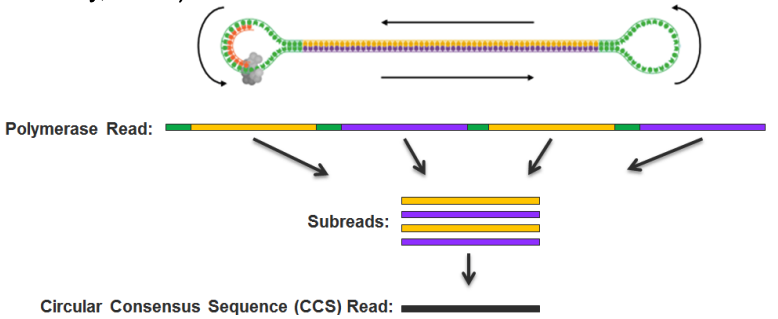
\includegraphics[width=0.65\textwidth]{CCS.png}
\par{Diagram outlining circular consensus sequencing (credit: PacBio website).}
\end{centering}
\end{figure}

\subsubsection{Linked reads}

\par{
The 10X platform starts with high molecular weight DNA input into a microfluidic system that partitions those long DNA molecules into GEMs (Gel bead in EMulsion) with oil surrounding an aqueous solution containing the DNA and reagents with a gel bead housing millions of copies of an oligo containing random primers, Illumina adapters, and the same barcode DNA sequence. Each different gel bead has a different barcode DNA sequence with high probability. Each GEM is poisson loaded with HMW DNA and on average gets roughly ten long molecules in the standard workflow. Short sequences are then amplified from these long molecules with random priming which creates a construct with the Illumina P5 and P7 adapters, the barcode oligo, and the DNA insert. This is then sequenced using standard short read Illumina sequencing. All of the reads with the same barcode sequence come from the same GEM and thus from a handful of long molecules. When the reads are mapped to a reference genome, the reads from each barcode cluster into a few small regions of the genome associated with their molecule of origin. This long range information can then be used to map into repeat regions of the genome, phase haplotypes, and call structural variation \cite{10xlinked}.
}

\begin{figure}[htbp!]

\caption{10x Genomics Linked reads}
\label{figure:linkedreads}
\begin{centering}
\sidesubfloat[]{
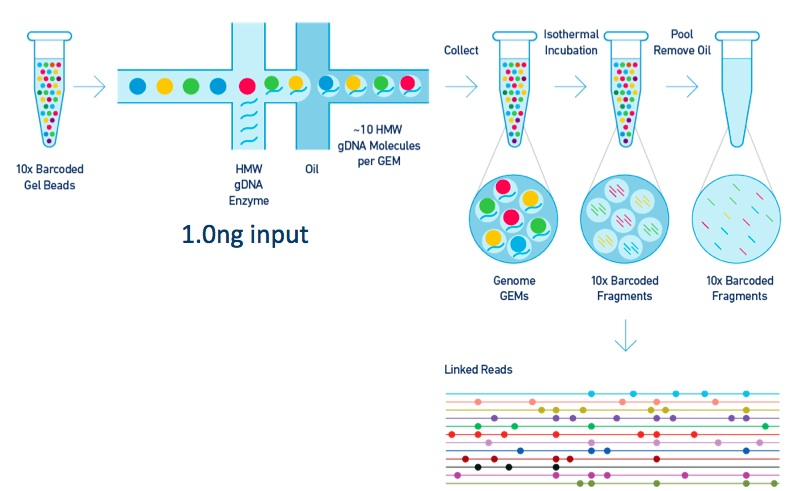
\includegraphics[width=0.65\textwidth]{linkedreads.jpeg} \label{fig:a}
} \\
\sidesubfloat[]{
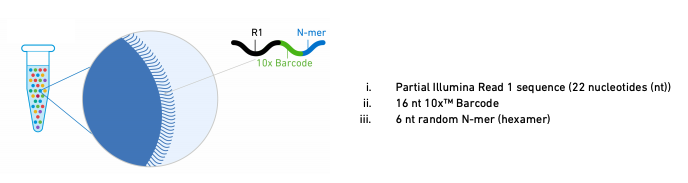
\includegraphics[width=0.65\textwidth]{gem.png} \label{fig:b}
} \\
\sidesubfloat[]{
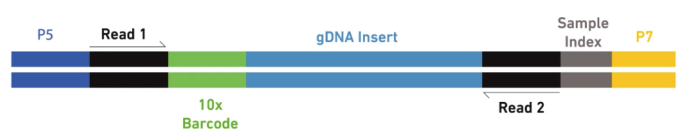
\includegraphics[width=0.65\textwidth]{construct.png} \label{fig:c}
}
\par{\textbf{a)} outlines the microfluidic system to create the Gel bead in reverse emulsion. \textbf{b)} shows the gel bead oligo setup and \textbf{c)} diagrams the final construct. (image credits to 10xgenomics website)}
\end{centering}
\end{figure}

\par{
While 10x Genomics Linked reads are used in Chapter 4, the technology is no longer offered by that company. More recently, bead based systems have been developed that do not require a microfluidic system. In solution with microbeads, long DNA molecules tend to wrap around a single bead\cite{beadphasing}\cite{LFR}. Separately, Tn5 transposase has been used to insert adapter and barcode sequences at high frequency into genomic DNA\cite{cptseq}. With these ideas combined, Frank Chan's group has developed a technique called Haplotagging which uses microbeads bound to Tn5 transposase with one of 85 million molecular barcodes and Illumina sequencing adapters creating linked read libraries for a fraction of the price in a single tube\cite{haplotagging}.
}

\subsubsection{High throughput chromatin conformation capture (Hi-C)}



\subsection{Reference Genomes}
\subsubsection{Resequencing}
\subsubsection{Read Mapping}
\subsubsection{Variant Calling}
\subsubsection{Population Genomics}

\subsubsection{The old way}
\subsubsection{The new way and Darwin Tree of Life and Earth Biogenome Project}

\subsection{Haplotype phasing}
\subsubsection{Statistical}
\subsubsection{Direct / Read based}

\subsection{Assembly}
\subsubsection{Overlap, Layout, Consensus}
\subsubsection{De brujin graphs}
\subsubsection{String graphs}
\subsubsection{Repeats, Heterozygosity, and Errors}
\subsubsection{Trio binning}
\subsubsection{Haploid assembly: Hytaditiform moles, seeds}
\subsubsection{Phased assembly}


\subsection{Post assembly manipulations}
\subsubsection{Polishing}
\subsubsection{Haplotig purging}
\subsubsection{Scaffolding}

\subsection{Assembly validation}
\subsubsection{Kmer based methods}
\subsubsection{Gene based methods}
\subsubsection{Contamination detection}

